%-*- coding=utf-8 -*-
\documentclass[UTF8]{ctexart}
\usepackage{geometry}
\CTEXsetup[format={\Huge\bfseries}]{section}
\CTEXsetup[format={\LARGE\bfseries}]{subsection}
%\usepackage{titlesec}
\geometry{left=3.18cm,right=3.18cm,top=2.54cm,bottom=2.54cm}
\usepackage{graphicx}
\pagestyle{plain}	
% \usepackage{booktabs}
% \usepackage{subfigure}
\usepackage{setspace}
\usepackage{float}
\begin{document}
	\begin{center}
		\quad \\
		\quad \\
		\heiti \fontsize{45}{17} 高级网络编程
		\vskip 2.0cm
		\heiti \fontsize{39}{17} 实验报告	
	\end{center}
	\vskip 3.5cm
	\begin{quotation}
		\par\setlength\parindent{8.5em}
		\quad 
		\heiti 
		
		实验名称:带有文件传输功能的多播聊天工具
		
		实验日期:2020年6月10日
	
		学生姓名:黄文政
		
		学\hspace{0.72cm}号:71Y17111
		
		\vskip 2cm
		\centering
	\end{quotation}
	
\newpage
\songti \fontsize{13}{13}
\large
\section*{一、实验目的}

用多播的方式实现1-N 的文字聊天(注:一定要用多播实现,做成聊天室的该项考核不合格),应能够支持:

1. 支持字符的传输,即聊天文本的传输;

2. 支持文件的传输,例如:源通过多播方式将文件(音视频)发送给多个接收方,接收方收到后,能够播放;

3. 能够对多播组成员进行管理;

4. 利用非对称密钥进行加密传输。

\section*{二、实验环境}

windows 10

qt 5.12.0

1920x1080分辨率

cryptopp 8.0.0

\section*{三、实验内容}
\subsection*{\textbf{1. 整体介绍}}
本软件实现了基于多播的文本聊天、音频文件传输的功能,并依靠单播实现了成员管理的功能。在传输过程中使用了
cryptopp对文本聊天和文件传输的内容进行加密解密,提高了软件的安全性。

软件运行的基本流程:在软件启动之初,需要向管理端申请唯一标识,并获取公钥密钥;随后会启动一个线程,定期
发送心跳信息,告知管理端和其他用户自身的存在;运行中可以执行文本聊天、文件传输、修改名称等功能;当用户
被管理端删除时,发送消息令该用户的程序退出,其他用户在一定周期内没有收到该用户的心跳信息,则认为该用户
已退出。

\subsection*{\textbf{2. 文本聊天}}
\subsection*{2.1 发送文本}
首先从UI中获取用户输入的文本内容,对文本内容进行加密,随后按如下结构构造信息包:

1. 标识符:“m”

2. 当前用户名字:字符串长度、字符串

3. 主要数据:加密内容

在信息包构造之后便以多播的方式发送出去。

\subsection*{2.2 接收文本}
接收到数据包后,查看标识符,若为“m”(文本聊天标识),则进行聊天文本的解析。先读取字符串长度,根据该值读
取发送人的昵称;剩下的信息则是加密后的文本内容。利用私钥对加密内容进行解密,获取解密内容,并显示在UI界
面上。

\begin{figure}[H]
\includegraphics[width=\textwidth]{pic/textchat.PNG}
\caption{文本聊天}
\end{figure}

\subsection*{\textbf{3. 音频文件传输}}
\subsection*{3.1 发送文件}
发送方选择要发送文件的完整路径,点击发送按钮之后,创建新的线程进行文件发送。

\begin{figure}[H]
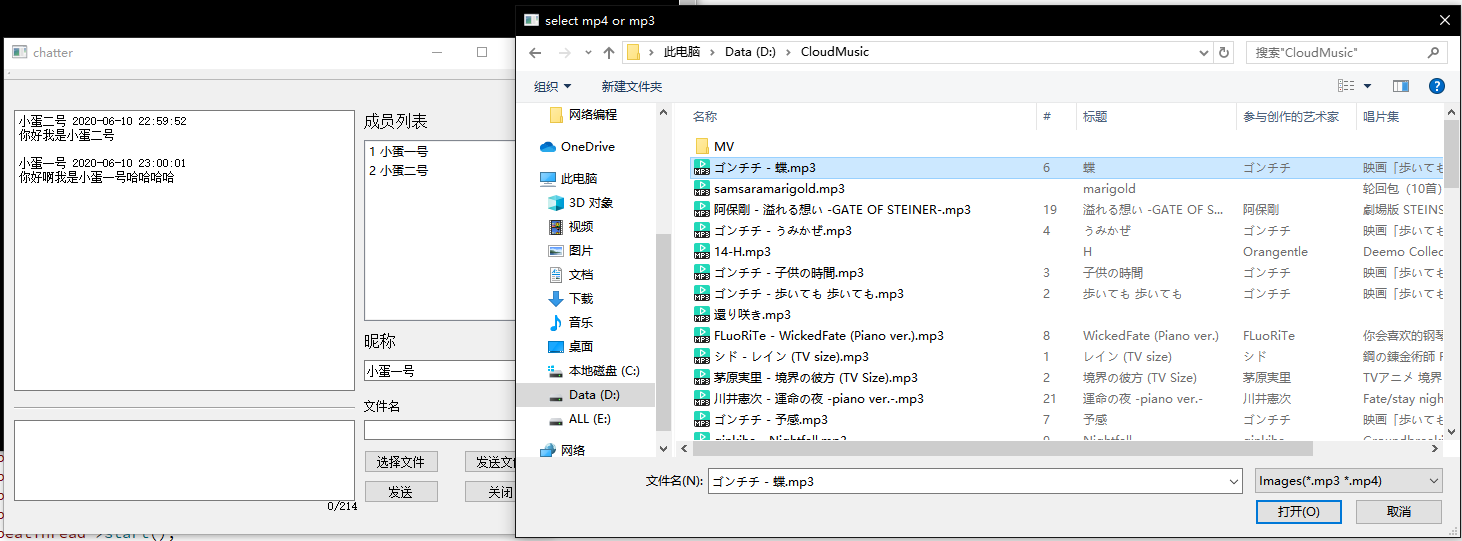
\includegraphics[width=\textwidth]{pic/filechoose1.PNG}
\caption{选择文件}
\end{figure}

首先发送开始包,包格式如下:

1. 标识符:“f”

2. 序号:0(qint64)

3. 剩余文件大小:(qint64)

4. 加密的文件名称

然后发送中间包,包含了加密的文件内容,包格式如下:

1. 标识符:“f”

2. 序号:(qint64)

3. 剩余文件大小:(qint64)

4. 加密的文件内容:(512bytes)

在将整个文件发送出去后,发送结束包,包格式如下:

1. 标识符:“f”

2. 序号:-1(qint64)

3. 剩余文件大小:0(qint64)

在整个发送流程完成后,结束线程、关闭文件。

\begin{figure}[H]
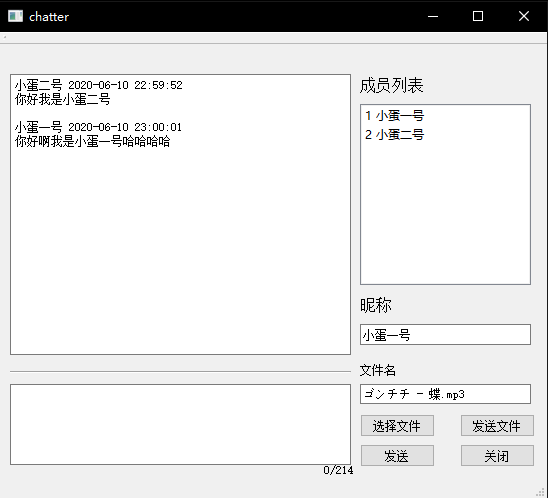
\includegraphics[width=\textwidth]{pic/filechoose2.PNG}
\caption{文件选择完成}
\end{figure}

\subsection*{3.2 接收文件}
接收方在接收到数据包后,查看标识符,若为“f”,则进行文件包的解析。

首先读取序号,若为开始包,则创建一个窗口进行接收进度展示;若为中间包,根据剩余文件大小更新接收进度,并将
解密的文件内容按照“序号-内容”的键值对保存在字典中;若为结束包,则可认为文件内容已全部接收完毕,按照接收
序号的顺序将文件内容写入硬盘中,并提供播放音频文件的按钮。利用这种方法可以有效解决UDP传输的乱序问题,但
丢包问题仍无法解决。

\begin{figure}[H]
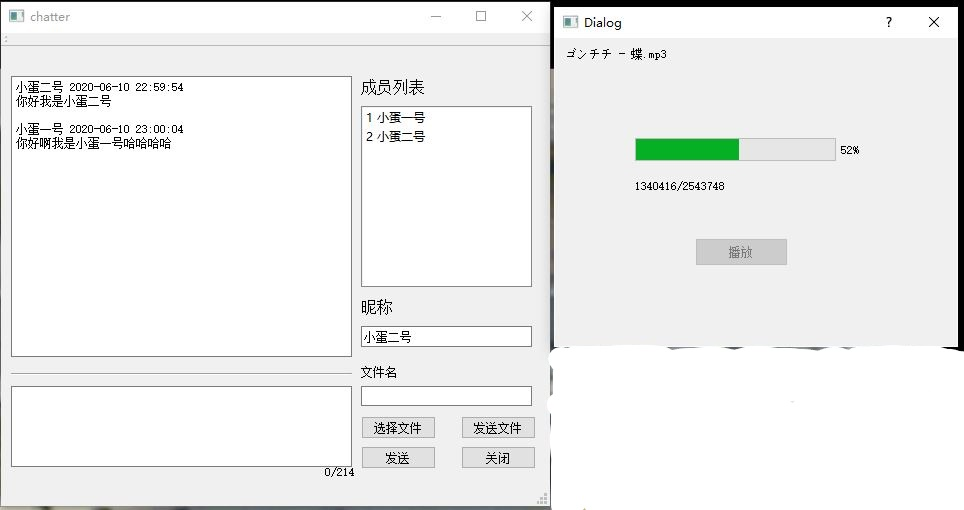
\includegraphics[width=\textwidth]{pic/filerecv1.jpg}
\caption{文件接收}
\end{figure}

\subsection*{3.3 播放音频}
文件接收完毕后,可以点击播放按钮进行播放。点击后会创建一个新的窗口,自动识别接收的是MP3还是MP4的文件,进
行音乐或视频的播放,并提供开始/暂停、通过进度条改变位置的常用播放功能。

\begin{figure}[H]
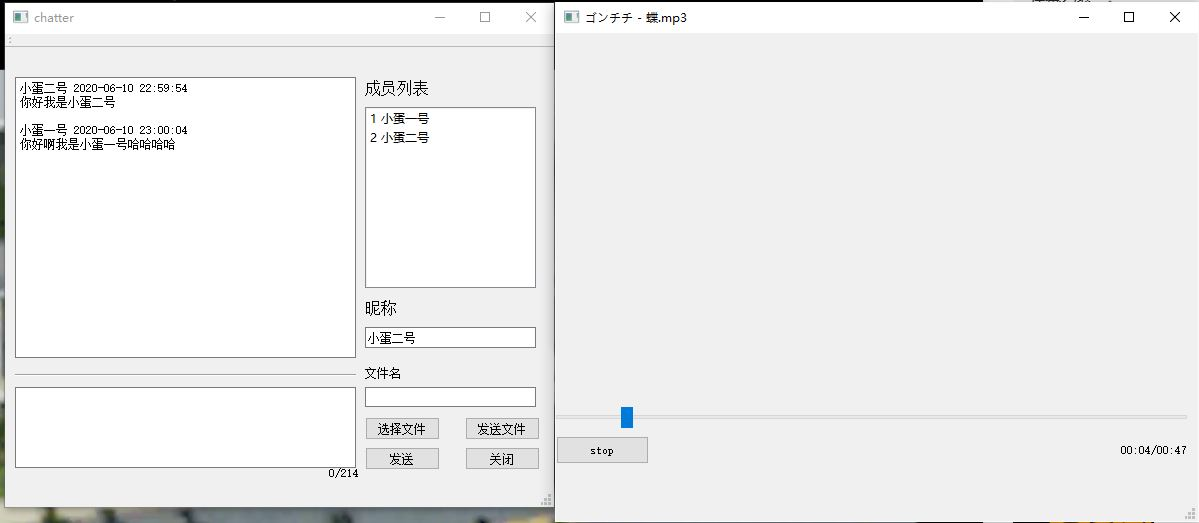
\includegraphics[width=\textwidth]{pic/MP3.JPG}
\caption{播放MP3}
\end{figure}

\begin{figure}[H]
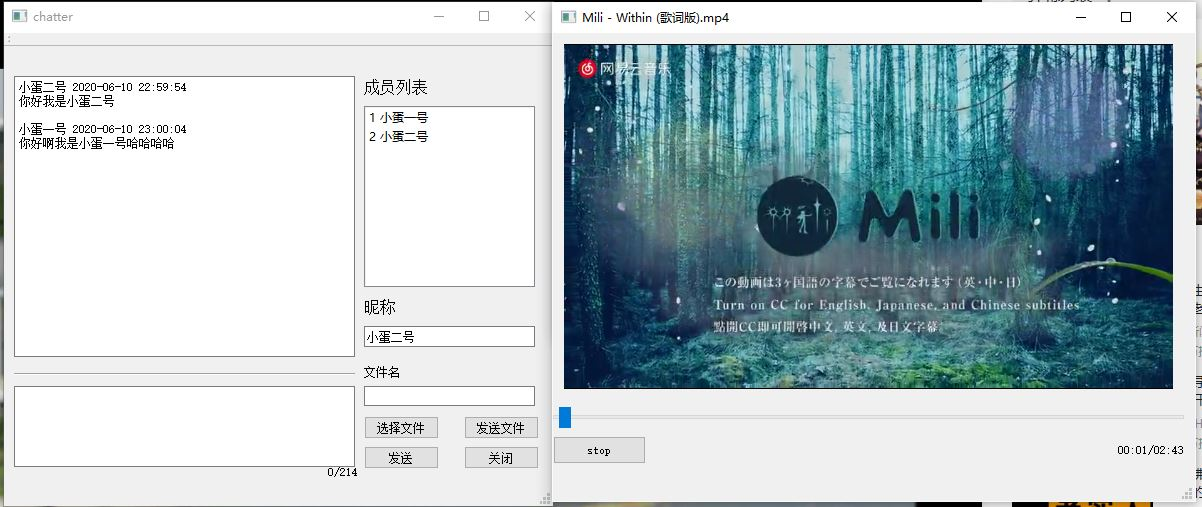
\includegraphics[width=\textwidth]{pic/MP4.JPG}
\caption{播放MP4}
\end{figure}

\subsection*{\textbf{4. 多播成员的管理}}
\subsection*{4.1 基于单播的管理}
每个用户在打开软件时,会向管理端申请唯一标识,作为管理端识别不同用户的依据,同时也允许了不同用户使用相同
的昵称。随后每个用户会定期以多播的形式发送心跳信息,其中包含了昵称、ID,管理端接收到之后将在线用户显示在
UI上。若在一定周期内未收到来自某一用户的心跳信息,则认为该用户已下线,从显示列表中删除该用户。

\subsection*{4.2 显示成员}
管理端在接收到用户的心跳信息后,便将用户的唯一标识、昵称、IP地址显示在UI界面上。每个已分配的用户标识都以
键值的形式存在字典中,其中键对应用户标识,值为距离上一次心跳响应的周期数。管理端在启动时会开启一个定时器,
每个周期结束后执行一个定时任务,增加每个用户标识距离上一次心跳响应的周期数,并检查是否超过5个周期,若超过
则认为该用户已下线,并释放该用户标识以供复用。

\begin{figure}[H]
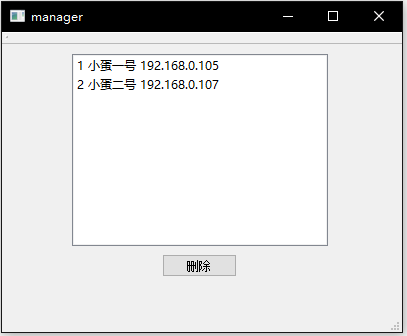
\includegraphics[width=\textwidth]{pic/userlist.PNG}
\caption{用户显示}
\end{figure}

\subsection*{4.3 删除成员}
管理端具有删除功能。利用鼠标单击选择一个用户后,点击删除按钮,便会对该用户软件发送删除命令,该用户的软件收
到该消息后会自动关闭聊天软件。

\begin{figure}[H]
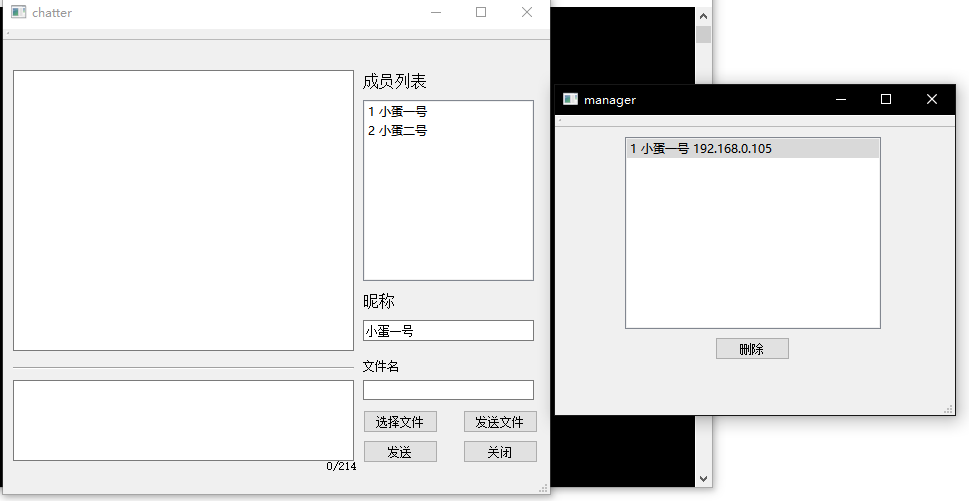
\includegraphics[width=\textwidth]{pic/deleteuser1.PNG}
\caption{点击删除按钮,未超过5个定时周期}
\end{figure}

\begin{figure}[H]
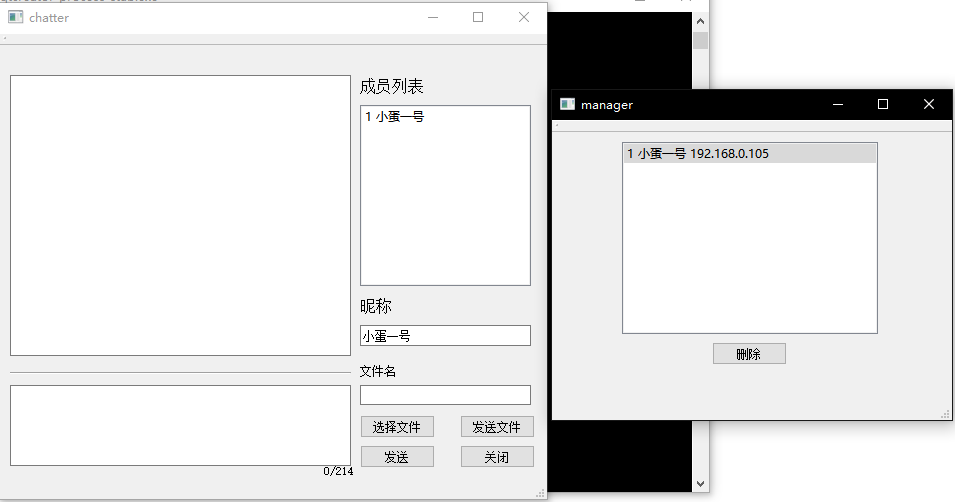
\includegraphics[width=\textwidth]{pic/deleteuser2.PNG}
\caption{点击删除按钮,超过5个定时周期}
\end{figure}

\subsection*{\textbf{5. 基于非对称的密钥加密}}
\subsection*{5.1 cryptopp}
cryptopp是一款免费的c++加密库,提供了多种常用的加密解密算法的接口。本次实验使用了cryptopp提供的RSA接口,
主要对字符串和二进制内容进行加密解密。

\subsection*{5.2 字符串的加密解密}
为了实现字符串的加密解密,利用crytopp提供的api封装了字符串加密解密函数,函数输入的参数为char类型的指针,
返回值为标准库string类型。在用户软件启动向管理端获取id的同时,还会向管理端获取公钥和密钥,作为加密传输的
基础。

\begin{figure}[H]
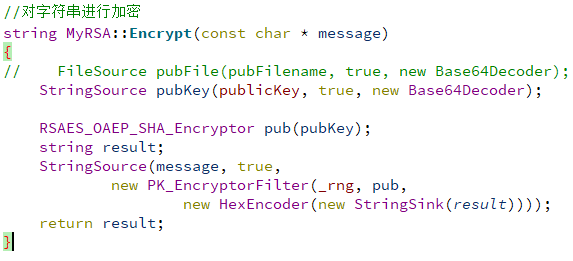
\includegraphics[width=\textwidth]{pic/strencrypt.PNG}
\caption{字符串加密函数}
\end{figure}

\begin{figure}[H]
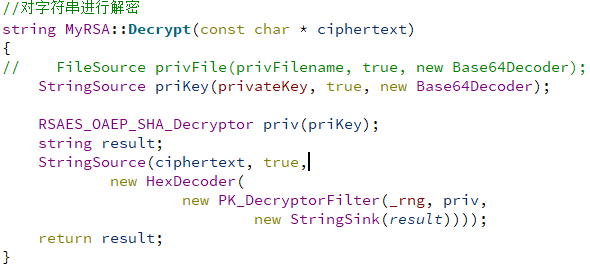
\includegraphics[width=\textwidth]{pic/strdecrypt.PNG}
\caption{字符串解密函数}
\end{figure}

\subsection*{5.3 二进制内容的加密解密}
由于二进制内容中可能包含“0”字符,这个字符在字符串中会被识别为终结符而造成后续信息的丢失,所以需要专门处理
二进制加密的函数。利用cryptopp提供的api封装了二进制内容加密解密的函数,函数输入的参数为源数据指针、源数据
长度、加密(解密)后数据指针、加密(解密)后数据长度。函数执行完成后通过加密(解密)后数据指针获取结果。在
用户软件启动向管理端获取id的同时,还会向管理端获取公钥和密钥,作为加密传输的基础。

\begin{figure}[H]
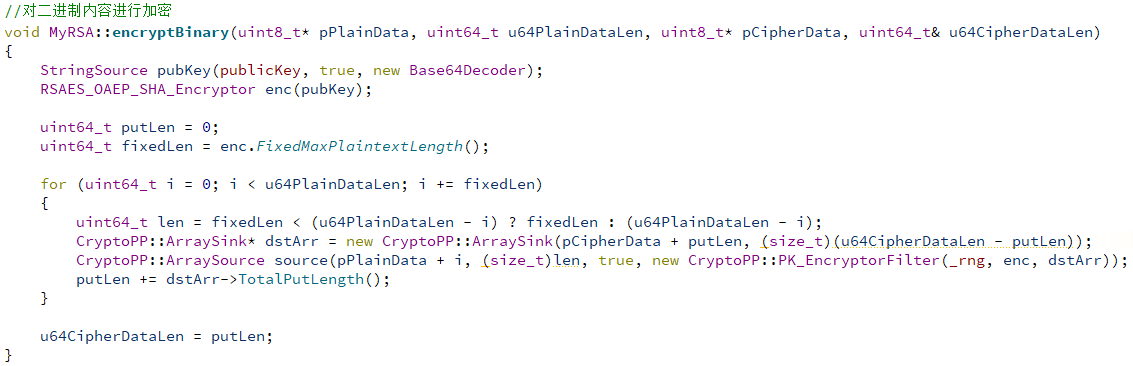
\includegraphics[width=\textwidth]{pic/binaryencrypt.PNG}
\caption{二进制内容加密函数}
\end{figure}

\begin{figure}[H]
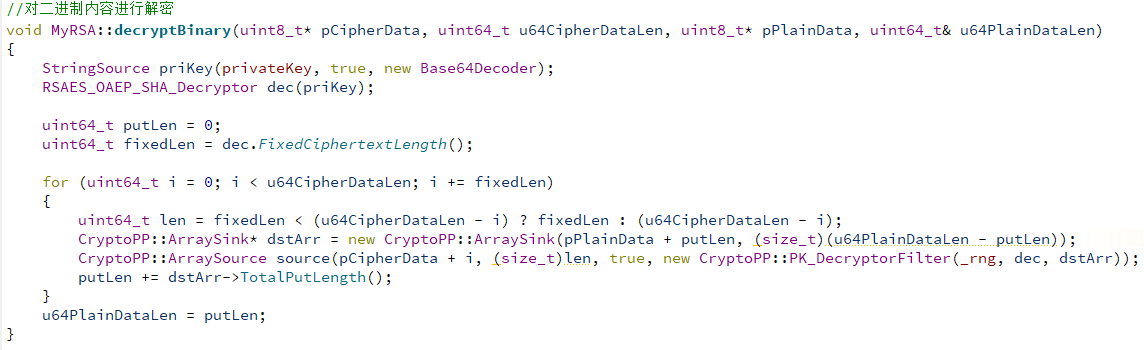
\includegraphics[width=\textwidth]{pic/binarydecrypt.PNG}
\caption{二进制内容解密函数}
\end{figure}

\section*{四、实验总结}
本次实验使用组播作为文本聊天、文件收发的网络信号传输方式,使用单播进行成员管理、公钥密钥的分配,并基于
cryptopp进行非对称加密传输的实现,基本完成了实验要求。

但软件还存在着一些问题。考虑到实验环境较差,单次发送网络包较大时易出现丢包问题,实验中采用了RSA2048进行加
密,单次发送的文本聊天信息包、文件信息包约为500字节,同时在发送文件时设置了每个包之间的发送间隔;而发送文
件也只能同时由一个用户发送,否则容易出现丢包问题。由于采用了单播进行成员管理的方法,一台主机只能运行一个用
户端,否则会出现端口重复绑定的问题。将来还可以从这些问题出发,寻找改进该软件的方法,使其更加稳定、可靠。

\end{document}